\documentclass[conference]{IEEEtran}

\usepackage{cite}
\usepackage{amsmath}
\usepackage{amssymb}
\usepackage{booktabs}
\usepackage{graphicx}
\usepackage{tikz}
\usetikzlibrary{positioning,arrows.meta}
\usepackage{url}

\title{Confidence-Aware QoE Routing for Multimedia Traffic in an SDN Testbed}

\author{\IEEEauthorblockN{Amit Nishad}
\IEEEauthorblockA{Student ID: 262IT002\\Department / Institution\\Email address}
\and
\IEEEauthorblockN{Nikhilesh Joshi}
\IEEEauthorblockA{Student ID: 262IT029\\Department / Institution\\Email address}
\and
\IEEEauthorblockN{Nikhil Bansal}
\IEEEauthorblockA{Student ID: 262IT028\\Department / Institution\\Email address}
\and
\IEEEauthorblockN{Shubham Joshi}
\IEEEauthorblockA{Student ID: 262IT033\\Department / Institution\\Email address}}

\begin{document}
\maketitle

\begin{abstract}
Multimedia traffic requires adequate throughput, low delay, and controlled packet loss. This project proposes AIRSDN, a software-defined networking approach for selecting a minimum-cost feasible route under bandwidth, delay, loss, and congestion constraints. The project presentation sets objectives for event-triggered rerouting, traffic-data collection and prediction, constrained shortest-path selection, and end-to-end system evaluation. The current Windows application demonstrates the NSFNET topology and a confidence-aware QoE routing simulation with deterministic scenario data; it does not yet implement every objective as a live network function. Accordingly, this report distinguishes the proposed design from implemented behavior and does not present fixture values as measured network performance.
\end{abstract}

\renewcommand{\IEEEkeywordsname}{Keywords}
\begin{IEEEkeywords}
software-defined networking, QoE, multimedia routing, confidence-aware routing, NSFNET, network simulation
\end{IEEEkeywords}

\section{Introduction}
\subsection{Problem Definition}
The project problem statement is to design an efficient constrained-optimization method that selects a minimum-cost path in a dynamic network while meeting bandwidth, delay, packet-loss, and congestion requirements \cite{airsdn_presentation}. Interactive video and similar multimedia applications need steady throughput, low delay, and limited loss. A short route may become congested, so a route decision should account for current path conditions. SDN separates forwarding from control and provides a controller that can configure paths using network-wide information \cite{kreutz2015sdn}.

\subsection{Importance of the Problem}
Multimedia quality depends on network conditions along the entire route. Selecting a path using delay, throughput, packet loss, jitter, and utilization can make routing decisions more informative than hop count alone. The supplied AIRSDN study provides the research context for applying AI-assisted routing to multimedia traffic \cite{ipek2025airsdn}.

\subsection{Challenges and Existing Solutions}
Static shortest-path routing is simple, but does not react to congestion. Controller-driven SDN makes network-wide path selection possible, although reliable decisions depend on fresh measurements and a functioning control plane. The current project addresses the decision logic in a deterministic simulation; it does not claim that its Windows demo is connected to live switches.

\subsection{Core Idea and Motivation}
AIRSDN evaluates a bounded set of loop-free candidate paths. It accepts a low-traffic prediction only when confidence reaches a threshold; otherwise it chooses the candidate with the strongest weighted QoE score. This provides a visible demonstration of confidence-aware routing and a fallback decision, while keeping future integration with measured telemetry possible.

\subsection{Project Objectives}
The presentation defines four objectives \cite{airsdn_presentation}: (1) design event-triggered rerouting that responds to congestion while limiting unnecessary path changes and service interruptions; (2) collect network data and develop a machine-learning traffic-prediction model; (3) investigate multi-constraint routing that minimizes transmission cost subject to bandwidth, delay, and packet-loss requirements; and (4) compare models, multimedia quality, backend services, and visualization as part of a final system evaluation.

\subsection{Project Contributions and Scope}
The current software contribution is a paper-aligned NSFNET topology, candidate path enumeration and validation, a confidence gate with QoE fallback, and a web visualization of decisions and packet progression. The objectives above describe the full project target; the live data-collection, trained-model, event-triggered flow-installation, and measured multimedia-evaluation stages remain future integration/evaluation work. The deterministic Windows demo is not a new trained model or a measured performance result.

\subsection{Report Organization}
Section II reviews the project context. Section III states the problem and objectives. Section IV describes the topology and proposed routing method, then distinguishes it from the current implementation. Section V reports the simulation fixture and evaluation plan. Section VI discusses complexity, limitations, and future directions.

\section{Literature Survey}
SDN separates the control plane from packet forwarding, allowing a logically centralized controller to configure paths using network state \cite{kreutz2015sdn}. This architecture is relevant to adaptive routing because forwarding decisions can be revised as link or traffic conditions change. The supplied AIRSDN paper studies AI-based routing for multimedia transmission and is the project's primary research reference \cite{ipek2025airsdn}.

The project adapts this motivation into a demonstration using candidate routes, traffic confidence, and QoE metrics. The implementation details reported here are specific to this project; the deterministic values in its demo should not be read as results from the cited paper. Mininet is a platform for creating virtual network topologies, while Floodlight is an SDN controller intended for OpenFlow environments \cite{mininet,floodlight}. They form the intended real-network integration environment, subject to the deployment requirements described below.

\subsection{Programmable Networks and Traffic Engineering}
SDN research describes the move from device-by-device configuration toward programmable control of forwarding behavior. OpenFlow provides a standardized controller-to-switch interface that supports experimental forwarding policies \cite{mckeown2008openflow}. Survey work identifies traffic engineering, controller placement, scalability, and reliability as continuing design questions in SDN \cite{hu2014sdn,nunes2014sdn}. For AIRSDN, the practical consequence is that a route-selection method must be paired with a safe actuation mechanism: a controller needs to install rules consistently, preserve reachability, and avoid changing a path faster than the network can converge.

\subsection{Learning-Assisted Routing and Traffic Classification}
Machine learning can support routing when labels or measurements expose patterns that are difficult to represent with a static link metric. For example, MLaR studies centralized link-state routing assisted by machine learning in software-defined wireless networks \cite{cicioglu2023mlar}. Traffic classification literature also emphasizes that feature choice, labeling quality, and the collection environment affect model quality. The AIRSDN research paper reports deriving a reduced set of 19 useful features from network-flow and path measurements, and compares several classifiers on its own simulated dataset \cite{ipek2025airsdn}. These studies motivate learning from telemetry but do not imply that a trained classifier is currently connected to this project's demo.

\subsection{AIRSDN Research Paper and Project Relationship}
The supplied paper evaluates an AI-based routing approach on an NSFNET-inspired Mininet topology. Its abstract reports 876 generated records, whereas its performance-results section reports 867; we preserve this discrepancy rather than silently choosing one count. The paper reports a 70\%/15\%/15\% train/validation/test split, Logistic Regression F1 score of 0.964, and AUC of 0.955. It also assesses video quality with PSNR and SSIM. These values belong to the cited paper and its dataset, not to the present project's fixture-based visualization \cite{ipek2025airsdn}. The current project adopts the topology and confidence-aware multimedia-routing motivation, then extends its stated project goals to include feasibility constraints and event-triggered rerouting. A future measured evaluation should therefore report its own dataset, split, controller configuration, and video-quality results.

Table~\ref{tab:related} summarizes the relationship between source literature and this implementation.
\begin{table}[t]
\centering
\caption{Research context and how it informs this project}
\label{tab:related}
\begin{tabular}{@{}p{0.27\columnwidth}p{0.62\columnwidth}@{}}
\toprule
Source & Relevance to AIRSDN \\
\midrule
SDN/OpenFlow surveys & Establish programmable control and the role of network-wide traffic engineering. \\
ML-assisted routing & Motivates learning from link-state and traffic measurements; models remain topology/data dependent. \\
AIRSDN multimedia study & Provides the NSFNET topology and multimedia routing research context; its published measurements are external results. \\
NFStream & Provides a cited flow-analysis framework suitable for a future data-collection pipeline. \\
\bottomrule
\end{tabular}
\end{table}

\section{Problem Statement and Objectives}
The problem is to select a minimum-cost route $p$ between source $s$ and destination $t$ in a dynamic network, subject to service constraints. The presentation's intended optimization can be written as
\begin{equation}
 \min_{p\in\mathcal{P}_{s,t}} C(p),\quad
 T(p)\geq B_{\mathrm{req}},\quad R(p)\leq R_{\max},\quad
 J(p)\leq J_{\max},\quad L(p)\leq L_{\max},
\end{equation}
where $\mathcal{P}_{s,t}$ is the set of candidate paths, $B_{\mathrm{req}}$ is the requested video bitrate, and $R,J,L$ denote RTT, jitter, and packet loss. A candidate must also be live and have fresh measurements \cite{airsdn_presentation}. The complete objective is constrained path selection, rather than simply minimizing hop count.

The four objectives are (1) event-triggered rerouting that reacts to congestion while minimizing unnecessary route changes and service interruption; (2) collection of network data and development of a traffic-prediction model; (3) investigation of constrained shortest-path methods for bandwidth, delay, and packet-loss requirements; and (4) comparison and evaluation of prediction models, multimedia quality, backend API, and visualization \cite{airsdn_presentation}.

Table~\ref{tab:objective_status} distinguishes these presentation objectives from the present demonstrator. This status description is included to avoid presenting planned work as already measured or deployed.
\begin{table}[t]
\centering
\caption{Relationship between presentation objectives and current project status}
\label{tab:objective_status}
\begin{tabular}{@{}p{0.48\columnwidth}p{0.42\columnwidth}@{}}
\toprule
Objective & Current status \\
\midrule
Event-triggered rerouting & Scenario changes are visualized; optimization to minimize real route churn is future work. \\
Data collection and ML model & Demo uses fixture confidence and metrics; live data/model inference is future work. \\
Multi-constraint routing & QoE ranking exists; bitrate and delay/loss feasibility constraints are not enforced in the demo. \\
System evaluation & UI and backend demo can be inspected; measured multimedia comparison remains future work. \\
\bottomrule
\end{tabular}
\end{table}

\section{Proposed Methodology}
\subsection{Network Topology}
Fig.~\ref{fig:topology} presents the topology encoded by the project. It has switches $S_0$--$S_{13}$ and 20 undirected inter-switch links. The receiver host is attached to $S_0$, while the sender/server host is attached to $S_9$. A Floodlight controller is shown as the SDN control-plane component. The same edge list is used by the software topology and the optional Mininet topology.

\begin{figure*}[t]
\centering
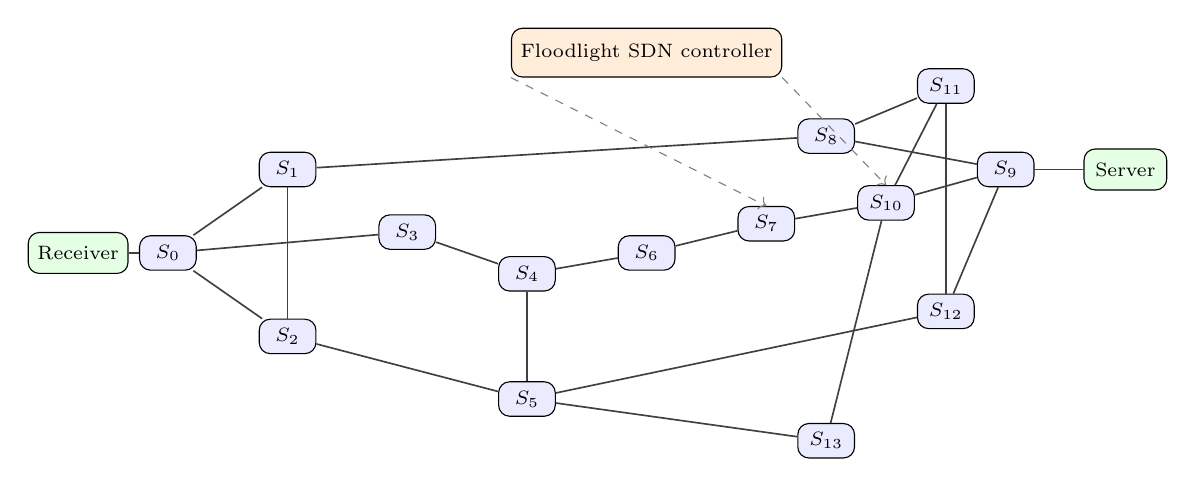
\begin{tikzpicture}[x=0.76cm,y=0.53cm,
  sw/.style={draw,rounded corners,fill=blue!8,minimum width=0.72cm,minimum height=0.42cm,font=\scriptsize},
  host/.style={draw,rounded corners,fill=green!10,minimum width=1.05cm,minimum height=0.52cm,font=\scriptsize},
  ctl/.style={draw,rounded corners,fill=orange!15,minimum width=1.55cm,minimum height=0.62cm,font=\scriptsize},
  link/.style={draw=black!75, line width=0.6pt}]
  \node[host] (rx) at (-1.5,0) {Receiver};
  \foreach \n/\x/\y in {0/0/0,1/2/2,2/2/-2,3/4/0.5,4/6/-0.5,5/6/-3.5,6/8/0,7/10/0.7,8/11/2.8,9/14/2,10/12/1.2,11/13/4,12/13/-1.4,13/11/-4.5}
    \node[sw] (s\n) at (\x,\y) {$S_{\n}$};
  \node[host] (srv) at (16,2) {Server};
  \node[ctl] (controller) at (8,4.8) {Floodlight SDN controller};
  \foreach \a/\b in {0/1,0/2,0/3,1/2,1/8,2/5,3/4,4/5,4/6,5/12,5/13,6/7,7/10,8/9,8/11,9/10,9/12,10/11,10/13,11/12}
    \draw[link] (s\a)--(s\b);
  \draw[link] (rx)--(s0);
  \draw[link] (s9)--(srv);
  \draw[dashed,->,gray] (controller.south west) -- (s7.north);
  \draw[dashed,->,gray] (controller.south east) -- (s10.north);
\end{tikzpicture}
\caption{AIRSDN NSFNET topology used in the project visualization. Solid lines are data links; dashed arrows indicate the logical controller relationship.}
\label{fig:topology}
\end{figure*}

The project topology includes multiple routes between the endpoints. Example routes include $S_0$--$S_1$--$S_8$--$S_9$ and $S_0$--$S_2$--$S_5$--$S_{12}$--$S_9$. The software enumerator performs depth-first search over simple paths, sorts candidates by hop count and node sequence, and returns up to five routes. This is exhaustive enumeration for this small graph, not a scalable k-shortest-path algorithm.

\subsection{Presentation Algorithm}
The presentation's target routing cycle obtains at most $K=5$ candidate paths. For each path it reads a telemetry snapshot, rejects missing, stale, or infeasible candidates, predicts the probability $q(p)$ of high traffic from scaled features, derives confidence $c(p)=\max(q(p),1-q(p))$, and calculates a normalized QoE proxy. The proposed logistic-regression probability is $q(p)=\sigma(\mathbf{w}^{T}\mathbf{x}(p)+b)$, where $\mathbf{x}$ contains the 19 classifier features. The slide deck uses throughput, RTT, jitter, and loss as principal path metrics. If any feasible path has a confidently low-traffic prediction, the selector considers only those paths; otherwise it considers all feasible paths. It maximizes QoE, breaking ties by fewer hops and then the earlier controller path index. The intended final operation installs forward and reverse flow rules. This is the proposed design in the presentation; the current Windows demo does not perform all of these live operations \cite{airsdn_presentation}.

The target feasibility filter requires a live path and fresh measurements. Throughput must meet the requested video bitrate, while RTT, jitter, and loss must satisfy configured limits. Let $F$ denote the feasible candidate set. The intended choice is
\begin{equation}
 p^*=\arg\max_{p\in S}Q(p),\qquad
 S=\begin{cases}A,&A\ne\emptyset,\\F,&A=\emptyset,\end{cases}
\end{equation}
where $A=\{p\in F:q(p)<0.5,\ c(p)\geq\epsilon\}$ is the set of confidently low-traffic routes, with $0.5<\epsilon<1$. The presentation leaves $\epsilon$ and the QoE weights to configuration. Its QoE proxy combines benefit-normalized throughput and cost-normalized RTT, jitter, and loss:
\begin{equation}
 Q(p)=w_Tn(T_p)+w_Rn(R_p)+w_Jn(J_p)+w_Ln(L_p),
 \quad w_T+w_R+w_J+w_L=1.
\end{equation}
For a benefit metric, $n(v)=\operatorname{clip}((v-a)/(b-a),0,1)$; for a cost metric, $n(v)=1-\operatorname{clip}((v-a)/(b-a),0,1)$, where $a,b$ are the candidate-set bounds.

\subsection{Current Simulation Decision}
The current Python demo uses deterministic low- and high-load scenario records instead of collected telemetry or a trained classifier. It normalizes throughput, latency, loss, jitter, and utilization and calculates
\begin{equation}
 Q_i=0.35n^{+}(T_i)+0.25n^{-}(L_i)+0.15n^{-}(P_i)
 +0.10n^{-}(J_i)+0.15n^{-}(U_i).
\end{equation}
When a fixture record is labeled low traffic and its confidence is at least 0.90, the implementation chooses the qualifying record with greatest confidence, using QoE as a tie-breaker. Otherwise it chooses the highest-QoE candidate, with fewer hops as a tie-breaker. The current demo does not enforce the presentation's bitrate/RTT/jitter/loss feasibility limits, calculate confidence from 19 features, run online optimization, or install live forward/reverse rules. Its decisions and packet animation are simulation behavior.

\begin{figure}[t]
\centering
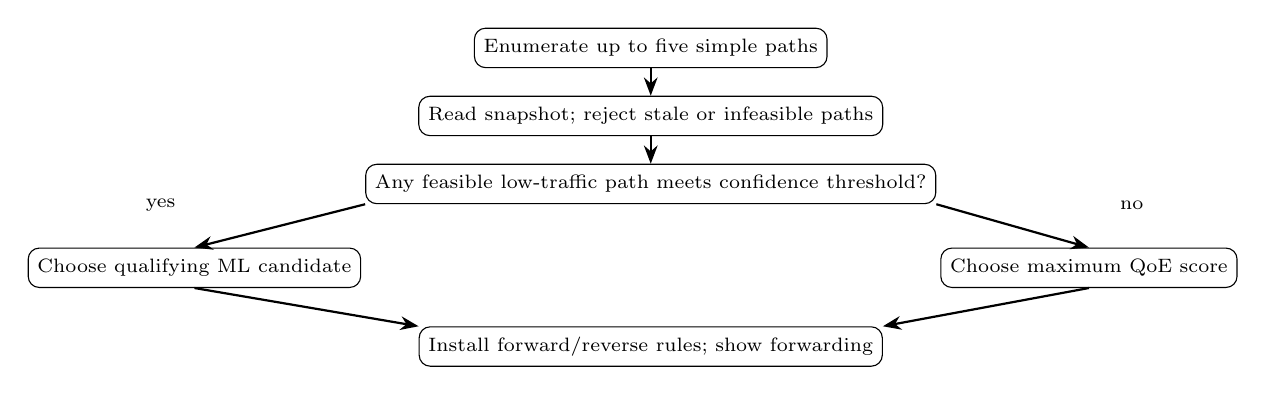
\begin{tikzpicture}[node distance=0.35cm, every node/.style={draw,rounded corners,align=center,font=\scriptsize,minimum width=3.0cm,minimum height=0.5cm}, arr/.style={-{Stealth},thick}]
\node (a) {Enumerate up to five simple paths};
\node[below=of a] (b) {Read snapshot; reject stale or infeasible paths};
\node[below=of b] (c) {Any feasible low-traffic path meets confidence threshold?};
\node[below left=0.55cm and 0.05cm of c] (d) {Choose qualifying ML candidate};
\node[below right=0.55cm and 0.05cm of c] (e) {Choose maximum QoE score};
\node[below=1.55cm of c] (f) {Install forward/reverse rules; show forwarding};
\draw[arr] (a)--(b); \draw[arr] (b)--(c);
\draw[arr] (c.south west)--node[above left,draw=none]{yes}(d.north);
\draw[arr] (c.south east)--node[above right,draw=none]{no}(e.north);
\draw[arr] (d.south)--(f.north west); \draw[arr] (e.south)--(f.north east);
\end{tikzpicture}
\caption{Simplified target route-selection flow from the presentation; live rule installation is not part of the current Windows demo.}
\label{fig:algorithm}
\end{figure}

\subsection{System Implementation}
The project is divided into a Python backend, a React/Vite visualization, and a network definition. The backend validates graph connectivity, enumerates routes, computes QoE scores, and returns a selected path and baseline comparison data. In the visualization, the operator can inspect the path candidates and algorithm stages; packet symbols traverse the chosen route when forwarding is enabled.

The Windows demonstration uses deterministic low- and high-traffic scenario fixtures to make the decision trace repeatable. Those fixture values are useful for demonstrating control flow, but they are not collected from a physical network, Mininet, or Floodlight. In the optional Mininet definition, hosts $h_0$ and $h_9$ attach to $S_0$ and $S_9$ respectively; host links are configured at 100 Mb/s and 1 ms, and inter-switch links at 100 Mb/s and 5 ms. Running that topology requires a Linux environment with Mininet and Open vSwitch. A live experiment additionally requires a reachable Floodlight controller and instrumentation to measure traffic.

\subsection{System Architecture}
The intended deployment has four cooperating layers. The data plane contains OpenFlow switches connected according to the NSFNET graph. The measurement layer observes flow counters, link state, RTT, loss, jitter, and throughput. A routing service on the control/application side constructs candidate paths, checks their feasibility, runs the prediction and QoE decision, and asks the controller to install the selected rules. The presentation layer displays topology, events, candidate metrics, and forwarding state. This separation makes it possible to test the decision module with synthetic input before connecting it to a controller.

In the present Windows setup, the Python backend and React visualization provide the simulated control and presentation path. The low/high scenario fixture supplies metric records; the API returns the topology and route decision; the browser visualizes selected-path forwarding. The diagram's controller and host links express the intended network design, while actual OpenFlow traffic requires a separately running Mininet/Open vSwitch/Floodlight environment. The project keeps that Linux integration path documented because these components are not replaced by the Windows browser simulation.

\subsection{Telemetry and Dataset Design}
A live observation should be associated with a timestamp, source/destination flow, candidate path, scenario label, and measurement interval. The project presentation groups 19 selected classifier features into a scaled feature vector $\mathbf{x}$ and a path-state vector $\mathbf{z}$ containing throughput, RTT, jitter, and packet loss. A robust collection pipeline should preserve raw observations as well as transformed values, record units, and mark a sample invalid when one of its required measurements is stale. NFStream provides a flow-statistics framework, while iperf3 and ping can generate traffic and measure capacity and round-trip behavior \cite{aouini2022nfstream}.

For supervised traffic prediction, the traffic label and feature interval must be defined before data collection. Training and test data should be separated by traffic run or scenario rather than by randomly splitting adjacent samples from the same flow. This reduces the chance that nearly identical measurements appear in both sets and makes the test closer to deployment on a new run. Feature scaling parameters must be fitted on training data only, then reused unchanged for validation and test inputs. Missing-value handling, class balance, and the high/low threshold must be recorded with the model artifact. A Logistic Regression model's confidence should be checked for calibration on held-out traffic; high classification accuracy alone does not guarantee reliable probability estimates \cite{alpaydin2020ml}.

The supplied research paper offers a useful precedent, not a substitute for project data: its dataset was generated under its own Mininet traffic scenarios, and its reported classifier results are tied to that dataset \cite{ipek2025airsdn}. The current project's fixture metrics are hand-authored scenario inputs and cannot be used to claim model training or generalization. A future AIRSDN experiment should archive a versioned CSV/Parquet dataset, feature dictionary, labeling rule, train/validation/test partition, and model parameters so the evaluation can be reproduced.

\subsection{Event-Triggered Rerouting Policy}
The project presentation identifies congestion-responsive rerouting with low route churn as an objective. A periodic controller poll can detect change, but rerouting at every small fluctuation may cause oscillation and service interruption. A proposed hysteresis policy is to switch only if the active route becomes infeasible, or if a different feasible route improves the QoE score by at least $\Delta_Q$ for $M$ consecutive measurement windows and a hold-down interval $T_h$ has expired. The thresholds $\Delta_Q$, $M$, and $T_h$ must be selected and reported during evaluation; they are not currently implemented in the Windows demo.

\begin{equation}
\text{switch if }\neg\mathrm{feasible}(p_{\mathrm{active}})\quad\text{or}\quad
\left[Q(p_{\mathrm{new}})-Q(p_{\mathrm{active}})\geq\Delta_Q\right]_{M\text{ windows}},
\quad t-t_{\mathrm{last}}>T_h.
\end{equation}
If a switch is needed, the controller should install and verify the new forward and reverse rules before removing the old rules where the platform permits make-before-break updates. If installation fails, it should retain or restore the last known working route and report the failure. These steps are a design recommendation derived from the presentation objective; the current backend does not manipulate live flow tables.

\subsection{Proposed Routing-Cycle Procedure}
The complete design can be expressed as a routing cycle. The following pseudocode describes the target integration and should not be confused with the current fixture-based implementation.
\begin{quote}\small\ttfamily
P := up to K candidate paths from s to t; F := empty; A := empty\\
for each p in P: read (features, metrics, timestamp, link state)\\
if sample is stale, path is down, or constraints fail: continue\\
q := logistic model(features); c := max(q, 1-q); score := normalized QoE\\
append (p, score) to F; if q < 0.5 and c >= epsilon: append p to A\\
if F is empty: report no feasible route\\
S := A if A is nonempty, otherwise F\\
p* := highest score in S; ties: fewer hops, then controller path order\\
if event trigger is satisfied: install and verify forward/reverse rules
\end{quote}
Candidate generation, snapshot validity, constraint filtering, model prediction, ranking, route-change hysteresis, and flow installation are separate operations. This separation helps isolate failures: a route may be absent because no candidate was returned, rejected because measurements are stale, or not installed because of a control-plane error.

\section{Experimental Results and Complexity Analysis}
\subsection{Simulation Results}
Table~\ref{tab:demo} summarizes representative scenario values configured in the current demo. They describe the chosen candidate in the deterministic fixture and should not be interpreted as measured performance. In the low-load case, the selected route passes the confidence gate. In the high-load case, the confidence is below the threshold and the QoE fallback is used.

\begin{table}[t]
\centering
\caption{Illustrative values from the deterministic demo fixture}
\label{tab:demo}
\begin{tabular}{@{}lcc@{}}
\toprule
Metric & Low scenario & High scenario \\
\midrule
Decision mode & ML routing & QoE fallback \\
Confidence & 0.96 & 0.86 \\
Selected path & 0--1--8--9 & 0--2--1--8--9 \\
Latency (ms) & 18 & 24 \\
Throughput (Mb/s) & 92 & 88 \\
Packet loss (\%) & 0.2 & 0.4 \\
\bottomrule
\end{tabular}
\end{table}

The dashboard can compare hop-count, QoS-aware, and AIRSDN choices for the same fixture. Such a comparison is a software demonstration of the implemented selection logic. A scientific performance claim would require repeated measured runs under controlled load, consistent traffic profiles, and uncertainty reporting. The supplied research article provides the motivation and research context; the values above are not a reproduction of its experimental results.

\subsection{Published Research Results for Context}
The source paper reports separate Mininet measurements under low- and high-traffic conditions. Table~\ref{tab:paper_results} reproduces selected values as contextual results from that publication only. The table is included to clarify the kind of outcomes a future project evaluation should measure; it is not a result produced by AIRSDN's current Windows demo \cite{ipek2025airsdn}.
\begin{table}[t]
\centering
\caption{Selected values reported by the supplied research paper}
\label{tab:paper_results}
\begin{tabular}{@{}lcc@{}}
\toprule
Measure & Low traffic & High traffic \\
\midrule
Mean RTT (ms) & 306.27 & 1710.59 \\
Packet loss (\%) & 0.00 & 13.99 \\
Bandwidth utilization (\%) & 33.18 & 93.31 \\
Throughput (Mb/s) & 6.68 & 0.67 \\
PSNR (dB) & 36.45 & 21.97 \\
SSIM & 0.996 & 0.917 \\
\bottomrule
\end{tabular}
\end{table}
These reported results illustrate why evaluating only route length is insufficient: under the paper's high-traffic scenario, latency, loss, utilization, throughput, and video quality all differ from the low-traffic scenario. They should not be numerically compared with this project's fixture table because the metrics, topology setup, generated traffic, and collection process are not shared experiments.

\subsection{Comparison and Evaluation Plan}
A next evaluation should run the topology in Mininet with a working OpenFlow controller, generate multimedia traffic, and collect throughput, round-trip delay, jitter, loss, and video-quality measures such as PSNR or SSIM where suitable. Each scenario should be repeated with a fixed seed and documented offered load. At minimum, compare shortest-hop routing, QoE-only selection, and confidence-aware AIRSDN using identical traffic traces. Report means and variability, and record controller and host configuration.

\subsection{Evaluation Metrics}
For a measurement interval of duration $\Delta t$, application throughput can be computed as delivered bits divided by $\Delta t$. Packet delivery ratio (PDR) is $N_{\mathrm{recv}}/N_{\mathrm{sent}}$, and packet-loss ratio is $1-\mathrm{PDR}$. The mean RTT is the arithmetic mean of valid echo or probe round trips in that interval. For successive one-way delay samples $d_i$, a simple jitter estimate is $\frac{1}{n-1}\sum_{i=2}^{n}|d_i-d_{i-1}|$; the exact estimator and clock source must be stated because jitter definitions vary across tools. Link utilization is measured bytes over interval divided by configured capacity over interval.

Video quality should be computed on decoded received frames aligned to the transmitted reference. PSNR is derived from mean squared pixel error, while SSIM compares local luminance, contrast, and structure. Reporting both is useful because a single pixel-error metric does not fully represent perceived structural similarity. The source study uses both measures; the project should use a consistent codec, resolution, frame rate, and alignment method across routing strategies \cite{ipek2025airsdn}.

For the binary traffic classifier, report confusion-matrix counts and class-wise precision and recall in addition to F1 and ROC-AUC. Precision is $TP/(TP+FP)$, recall is $TP/(TP+FN)$, and the harmonic mean is $F_1=2PR/(P+R)$. If the model confidence drives route selection, probability calibration and false-low predictions are especially important: a false-low prediction can cause the selector to trust a path that is congested. Results should include per-class metrics, not accuracy alone.

\subsection{Experiment Matrix}
Table~\ref{tab:experiment} gives a proposed controlled comparison. All strategies should use identical traffic traces and initial flow state. Link failures should be injected at a specified time and recovered after a fixed duration so recovery time and route churn can be compared. Every run should record the seed, offered bit rate, flow duration, topology, controller version, and sampling interval.
\begin{table}[t]
\centering
\caption{Proposed evaluation matrix}
\label{tab:experiment}
\begin{tabular}{@{}p{0.26\columnwidth}p{0.34\columnwidth}p{0.31\columnwidth}@{}}
\toprule
Scenario & Routing strategies & Primary observations \\
\midrule
Baseline load & Hop-count; QoE; AIRSDN & Throughput, RTT, loss, QoE \\
Traffic surge & Same strategies with rising offered load & Congestion response, reroute time, route changes \\
Link down/recovery & Link-state route exclusion and restoration & Reachability, packet interruption, recovery time \\
Multimedia transfer & Same video and codec over each route & PSNR, SSIM, delivered frames, bitrate \\
Model evaluation & LR and selected comparison classifiers & Precision, recall, F1, AUC, calibration \\
\bottomrule
\end{tabular}
\end{table}

The experiment should include multiple independent repetitions. For each metric, report the number of runs, mean, standard deviation, and a confidence interval; show per-run values where practical. The path chosen at startup and each subsequent route change should be logged with the reason, candidate scores, and telemetry timestamps. This makes an apparent QoE improvement auditable and helps identify cases where route installation or measurement lag, rather than the scoring rule, caused a poor outcome.

\subsection{Research Questions and Expected Comparisons}
The evaluation can be organized around four questions. RQ1 asks whether a route selected with current path metrics improves multimedia delivery relative to hop-count routing under the same traffic. RQ2 asks whether confidence-aware fallback avoids selecting a route on an unreliable low-load prediction. RQ3 asks whether feasibility constraints prevent the selector from choosing a route that cannot meet the requested bitrate or delay/loss limits. RQ4 asks whether an event trigger with hysteresis reduces unnecessary route changes without materially delaying response to real congestion or failure.

These are questions, not findings. For RQ1, compare throughput, RTT, packet loss, jitter, PSNR, and SSIM. For RQ2, measure calibration and error cases around the confidence threshold, along with routing outcomes. For RQ3, count constraint violations and no-feasible-path events. For RQ4, measure route changes per minute, time from a threshold crossing to a route update, packet interruption during transition, and recovery time after link restoration. The measurement interval and definitions must be fixed before interpreting differences.

\subsection{Operational Failure Handling}
In a live deployment, telemetry should carry a validity state and age. A route is not considered feasible when the measurement age exceeds a configured maximum, a required metric is missing, or a switch/link is reported down. The controller should distinguish ``no feasible candidate'' from ``measurement unavailable'' and ``rule installation failed'' in its logs. These outcomes have different remedies and should not be collapsed into a default route score.

Flow updates also require careful handling. A path change must update every switch on the forward and reverse directions, and stale rules should be removed only after the replacement is confirmed. If the controller loses a switch during installation, the application should detect partial installation and return to a known safe state. In addition, controller REST endpoints should be restricted to trusted hosts and protected according to the lab's security policy. These reliability and security controls are requirements for the Linux integration stage; the simulation API does not exercise them.

\subsection{Limitations}
Current limitations are the deterministic candidate telemetry, absence of live packet measurement in the Windows demo, and small-graph simple-path enumeration. The confidence input is not presently generated by a trained model in this demo. Future work includes connecting measured telemetry and classifier inference to the decision engine, installing selected flows through Floodlight, and validating the visualization against captured packet counters.

\subsection{Complexity Analysis}
The current path enumerator uses depth-first search over simple paths. Its worst-case running time is exponential in the number of vertices because the number of simple paths can grow exponentially; the implementation limits its returned results to five after enumeration. For this 14-switch demonstration topology, that approach is manageable, but a larger network should use a dedicated k-shortest-path method or a bounded search. QoE scoring for $k$ returned candidates takes $O(k)$ time and $O(k)$ storage.

The project presentation gives a post-path-retrieval routing-cycle estimate of $O(K(H+d+m)+H)$, where $K$ is the number of candidate paths, $H$ is the maximum path length, $d$ is the classifier feature count, and $m$ is the number of path metrics \cite{airsdn_presentation}. This estimate covers per-candidate validation, feature processing, prediction, and scoring under the presentation's assumed model. It does not include candidate-path generation; the current DFS enumerator can dominate runtime as topology size grows.

\subsection{Route Cost and Change Penalty}
The presentation frames the problem as minimum-cost routing, while its selection pseudocode ranks paths by normalized QoE. A consistent interpretation on the feasible set is $C_{\mathrm{route}}(p)=1-Q(p)$, so minimizing the normalized cost is equivalent to maximizing QoE. To express the stated objective of avoiding excessive route changes, a future controller can add a change penalty: $C_{\mathrm{decision}}(p)=1-Q(p)+\lambda\,\mathbb{I}[p\ne p_{\mathrm{active}}]$, where $\lambda$ represents the cost of a route change. This is a proposed formalization; neither the penalty nor the hysteresis threshold is present in the current simulation. The design should report $\lambda$ and evaluate the resulting trade-off between path quality and route stability.

\subsection{Threats to Validity}
Several limitations affect how results can be interpreted. First, the current implementation uses deterministic fixture metrics, so it does not demonstrate the accuracy of a model or the performance of a network. Second, normalized QoE is only a proxy for user experience; actual quality depends on the codec, buffering, frame rate, and application behavior. Third, the test topology is small and fixed, so path-enumeration cost and route diversity may differ in larger or wireless networks. Fourth, simulated packet animation is not packet capture evidence. Finally, a single traffic profile or run would not support statistical claims. These limitations can be reduced through live measurements, video-level metrics, independent runs, and external test topologies, but they cannot be removed by the visualization alone.

\subsection{Reproducibility and Deployment Modes}
The repository supports two distinct execution modes. The Windows mode runs a software simulation: from the repository root, execute \verb|.\setup_windows.ps1|, then start \verb|.\run_backend_windows.ps1| and \verb|.\run_frontend_windows.ps1| in separate PowerShell windows. The visualization is served at \url{http://localhost:5173/visualization}; the Python API listens on port 8000. The current server exposes \texttt{/api/health}, \texttt{/api/demo?scenario=low|high}, and \texttt{/api/stream?scenario=...\&forwarding=true}. The stream response labels its mode as simulation and returns packet-progress records along the selected path when forwarding is enabled. These are visual records, not packets emitted into Mininet.

The Linux integration mode requires Mininet, Open vSwitch, and an available Floodlight controller. The topology source is \texttt{network/nsfnet\_topology.py}; it defines switches \texttt{s0}--\texttt{s13}, receiver \texttt{h0}, server \texttt{h9}, 100 Mb/s host links with 1 ms delay, and 100 Mb/s inter-switch links with 5 ms delay. A reproducible live run should record controller version, switch protocol, topology revision, host kernel, traffic-generator version, and all scenario parameters. The API and integration scripts should fail closed or expose invalid telemetry when a dependency is unavailable rather than substituting synthetic numbers. Mininet and Floodlight provide the intended emulation and control-plane components \cite{mininet,floodlight}.

For repeatability, each evaluation run should have an experiment identifier that follows the generated traffic, telemetry rows, model output, route decision, and final video file. The log should retain timestamps, route before and after, reason for change, path metrics, model version, controller response, and whether flow rules were confirmed. This enables a reviewer to trace a plotted metric back to its source observations and distinguish measurements from display updates.

\section{Conclusion and Future Directions}
This report describes an AIRSDN prototype whose visualization uses the paper-aligned 14-switch topology and whose route selector combines a confidence gate with weighted QoE fallback. The current implementation provides a repeatable simulation for inspecting candidate paths and decisions. Its scenario numbers are illustrative fixture data, so claims about real network gains must wait for a measured Mininet/Floodlight experiment. Future work is to connect live telemetry and model inference, install selected flows through Floodlight, and compare routing strategies using repeated measured multimedia runs.

\appendices
\section{Experiment Record Schema}
The following record schema is a proposal for the future measurement pipeline. It separates identifiers and provenance from numeric features and derived decisions. Raw values and their units should be kept alongside normalized values so that a later analysis can recompute scores without guessing the original scale.

\begin{table}[t]
\centering
\caption{Recommended fields for one candidate-path observation}
\label{tab:record_schema}
\begin{tabular}{@{}p{0.28\columnwidth}p{0.60\columnwidth}@{}}
\toprule
Field group & Example contents \\
\midrule
Run identity & Experiment ID, run seed, scenario, timestamp, topology revision \\
Path identity & Source, destination, ordered switch IDs, hop count, controller path index \\
Link state & Per-link status, capacity, measured utilization, validity and sample age \\
Telemetry & Throughput, RTT, jitter, loss, units, observation interval \\
Classifier & Feature-vector version, traffic label, predicted probability, confidence, model version \\
Decision & Feasible flag, rejection reason, QoE score, chosen route, trigger reason \\
Actuation & Controller response, installed switches, rule verification, rollback status \\
Application quality & Video ID, codec, resolution, sent/received frames, PSNR, SSIM \\
\bottomrule
\end{tabular}
\end{table}

Every value should be traceable to a measurement source. For example, the telemetry record should identify whether RTT came from an ICMP probe or an application measurement, whether throughput represents interface bytes or iperf3 goodput, and whether packet loss was measured from the flow or inferred from a probe. A null value must remain null with a reason code; replacing missing observations with zero would incorrectly make an unavailable metric appear optimal or catastrophic depending on its direction.

\section{Demonstration and Experiment Checklist}
For the deterministic Windows demonstration, the operator can start the backend and frontend using the repository's PowerShell launchers, confirm the health endpoint, select low or high scenario, and inspect the topology, candidate list, confidence rule, QoE fallback, baselines, and stream state. A screenshot or screen recording should label this clearly as simulation mode. The event history should capture the selected scenario and path so that the explanation can be repeated consistently.

For a Linux experiment, first verify that Mininet hosts can reach each other and that every OpenFlow switch is connected to Floodlight. Confirm that the chosen source and destination match $h_0$ and $h_9$ and that the graph links match the paper-aligned edge list. Next collect baseline path metrics without rerouting, validate the measurement pipeline, and confirm the media file can be compared before and after transmission. Only after those checks should the event trigger and route installer be enabled. This staged procedure separates environment faults from routing-algorithm behavior.

Before reporting a result, retain the configuration file, software versions, topology edge list, dataset partition, random seeds, all run logs, and generated video-quality measurements. The report should state the number of independent runs and any failed runs with their failure reason. If a result changes after dropping a failed run, both the original and filtered counts should be disclosed. This evidence makes the final comparison reproducible and prevents a dashboard visualization from being mistaken for an instrumented network measurement.

\bibliographystyle{IEEEtran}
\bibliography{airsdn_references}
\end{document}
